\section{Black-Scholes公式}
\begin{enumerate}[label=\arabic{section}.\arabic*]
    \item \sol\\
    因为$\displaystyle \ln\left(\frac{S(t)}{S(0)}\right) \sim N\left(\left(r-\frac{\sigma^2}{2}\right)t,\sigma^2t\right)$,所以$\displaystyle \ln\left(\frac{S(t_1)}{S(t_2)}\right) \sim N\left(\left(r-\frac{\sigma^2}{2}\right)(t_1-t_2),\sigma^2(t_1-t_2)\right)$.
    \begin{enumerate}[label=\alph*)]
        \item $\displaystyle \sigma_d=0.33\sqrt{\frac{n-(n-1)}{365}}=0.0173$.
        \item $\displaystyle \sigma_m=0.33\sqrt{\frac{n-(n-1)}{12}}=0.0953$.
    \end{enumerate}
    \item \sol\\
    $\displaystyle t=\frac{4}{12}=\frac{1}{3}$,所以期权被执行当且仅当$\displaystyle S\left(\frac{1}{3}\right)>42$,而$\displaystyle \ln\frac{S(1/3)}{S(0)} \sim N\left(0.04,0.0192\right)$则
    \begin{align*}
        P\left[S\left(\frac{1}{3}\right)>42\right]&=P\left[\frac{S(1/3)}{S(0)}>\frac{42}{40}\right]=P\left[\ln\frac{S(1/3)}{S(0)}>\ln1.05\right]\\
        &=P\left(Z>\frac{\ln1.05-0.04}{\sqrt{0.0192}}\right)=1-\Phi(0.0634)\\
        &=1-0.5253=0.4747
    \end{align*}
    \item \sol\\
    本题中的参数为\[t=\frac{1}{3},r=0.08,\sigma=0.24,K=42,S(0)=40,\]
    则\[\omega=\frac{rt+\sigma^2t/2-\ln[K/S(0)]}{\sigma\sqrt{t}}=\frac{0.08/3+0.24^2/6-\ln(42/40)}{0.24/\sqrt{3}}=-0.0904,\]
    而$\Phi(-0.0904)=0.4640,\Phi(-0.2290)=0.4094$,所以
    \[C=S(0)\Phi(\omega)-K\e^{-rt}\Phi(\omega-\sigma\sqrt{t})=40\times0.4640-42\e^{-0.08/3}\times0.4094=1.8177.\]
    \item \sol\\
    由看跌-看涨期权平价公式,则
    \begin{align*}
        P&=C-S(0)+K\e^{-rt}=S(0)\Phi(\omega)-K\e^{-rt}\Phi(\omega-\sigma\sqrt{t})-S(0)+K\e^{-rt}\\
        &=S(0)[\Phi(\omega)-1]+K\e^{-rt}[1-\Phi(\omega-\sigma\sqrt{t})]
    \end{align*}
    本题中的参数为\[t=\frac{1}{2},r=0.10,\sigma=0.30,K=100,S(0)=105,\]
    则\[\omega=\frac{rt+\sigma^2t/2-\ln[K/S(0)]}{\sigma\sqrt{t}}=\frac{0.1/2+0.3^2/4-\ln(100/105)}{0.3/\sqrt{2}}=0.5718,\]
    而$\Phi(0.5718)=0.7163,\Phi(0.3596)=0.6404$,所以
    \[P=105\times(0.7163-1)+100\e^{-0.1/2}\times(1-0.6404)=4.4177.\]
    \item \sol {\kaishu \textcolor{blue}{注意:b)问少了一个条件:假设$r=0.05$.}}
    \begin{enumerate}[label=\alph*)]
        \item \begin{align*}
            P\left[\frac{S(0.5)}{S(0)}<0.9\right]&=P\left[\ln\frac{S(0.5)}{S(0)}<\ln0.9\right]=P\left(Z<\frac{\ln0.9-0.03}{\sqrt{0.3^2\times0.5}}\right)\\
            &=\Phi(-0.6381)=1-\Phi(0.6381)=1-0.7383=0.2617
        \end{align*}
        \item $\displaystyle r-\sigma^2/2=0.05-0.045=0.005$,与a)问类似,
        \begin{align*}
            P\left[\frac{S(0.5)}{S(0)}<0.9\right]&=P\left[\ln\frac{S(0.5)}{S(0)}<\ln0.9\right]=P\left(Z<\frac{\ln0.9-0.0025}{\sqrt{0.3^2\times0.5}}\right)\\
            &=\Phi(-0.5085)=1-\Phi(0.5085)=1-0.7383=0.3056
        \end{align*}
        投资的收益为\[\begin{cases}
            100\e^{-rt}-A, & \text{概率为}0.3056 \\ -A, & \text{概率为}0.7383
        \end{cases}\]
        所以\[E(\text{收益})=0.3056(100\e^{-0.025}-A)-0.7383A=0 \Rightarrow A=29.8055.\]
    \end{enumerate}
    \item \sol
    \begin{enumerate}[label=\alph*)]
        \item 本题中的参数为\[t=\frac{1}{4},r=0.04,\sigma=0.3,K=100,S(0)=95,\]
        则\[\omega=\frac{rt+\sigma^2t/2-\ln[K/S(0)]}{\sigma\sqrt{t}}=\frac{0.04/4+0.3^2/8-\ln(100/95)}{0.3/\sqrt{4}}=-0.2003,\]
        而$\Phi(-0.2003)=0.4206,\Phi(-0.3503)=0.3631$,所以
        \[C=S(0)\Phi(\omega)-K\e^{-rt}\Phi(\omega-\sigma\sqrt{t})=95\times0.4206-100\e^{-0.04/4}\times0.3631=4.0083.\]
        \item \begin{align*}
            P[S(1/4)<100]&=P\left[\frac{S(1.4)}{S(0)}<\frac{100}{95}\right]=P\left[\ln\frac{S(1.4)}{S(0)}<\ln\frac{100}{95}\right]\\
            &=P\left(Z<\frac{\ln(100/95)-0.05/4}{\sqrt{0.3^2/4}}\right)\\
            &=\Phi(0.2586)=0.6020
        \end{align*}
        \item $\displaystyle r-\frac{\sigma^2}{2}=-0.005$,下计算$P[S(1)>105]$,
        \[P[S(1)>105]=P\left(Z>\frac{\ln(105/95)+0.005}{0.3}\right)=1-\Phi(0.3503)=0.3631,\]
        再计算$P[S(1)>S(0.5)]$,\[P[S(1)>S(0.5)]=P\left(Z>\frac{0+0.005/2}{0.3/\sqrt{2}}\right)=1-\Phi(0.0118)=0.4953,\]
        则$0.3631 \times 0.4953=0.1798$,而收益为
        \[\begin{cases}
            50\e^{-rt}-C, & \text{概率为}0.1798\\-C, & \text{概率为}1-0.1798
        \end{cases}\]
        所以\[E(\text{收益})=0.1798(50\e^{-0.04}-C)-(1-0.1798)C=0 \Rightarrow C=0.1798\times50\e^{-0.04}=8.6375.\]
    \end{enumerate}
    \item \sol\\
    本题中的参数为\[t=\frac{1}{2},r=0.06,\sigma=0.32,K=40,S(0)=38,F=100,\]
    $\displaystyle r-\frac{\sigma^2}{2}=0.0088$,下计算$P[S(1/2)>K]$,
    \[P[S(1/2)>K]=P\left(Z>\frac{\ln(40/38)-0.0088/2}{\sqrt{0.32^2/2}}\right)=1-\Phi(0.2072)=0.4179,\]
    收益为
    \[\begin{cases}
        F\e^{-rt}-C, & \text{概率为}0.4179\\-C, & \text{概率为}1-0.4179
    \end{cases}\]
    所以
    \[E(\text{收益})=0.4179(100\e^{-0.06/2}-C)-(1-0.4179)C=0 \Rightarrow C=0.4179\times100\e^{-0.03}=40.5549.\]
    \item \sol\\
    本题中的参数为\[t=\frac{1}{2},r=0.06,\sigma=0.32,K=40,S(0)=38,F=100,\mu=0,\]
    $\displaystyle r-\frac{\sigma^2}{2}=0.0088$,下计算$P[S(1/2)>K]$
    \[P[S(1/2)>K]=P\left(Z>\frac{\ln(40/38)-0}{\sqrt{0.32^2/2}}\right)=1-\Phi(0.2267)=0.4179,\]
    收益为
    \[\begin{cases}
        F\e^{-rt}-C, & \text{概率为}0.4103\\-C, & \text{概率为}1-0.4103
    \end{cases}\]
    所以
    \[E(\text{收益})=0.4103(100\e^{-0.06/2}-C)-(1-0.4103)C=0 \Rightarrow C=0.4103\times100\e^{-0.03}=39.8174.\]
    \item \sol\\ 否,还需要知道几何布朗运动的漂移参数$\mu$.
    \item \sol
    \begin{enumerate}[label=\alph*)]
        \item $\displaystyle r-\frac{\sigma^2}{2}=-0.02$,下计算$P[S(1)<95]$,
        \[P[S(1)<95]=P\left(Z<\frac{\ln(95/100)+0.02}{\sqrt{0.4^2}}\right)=\Phi(-0.0782)=0.4688,\]
        再计算$P[S(1)>110]$,
        \[P[S(1)>110]=P\left(Z>\frac{\ln(110/100)+0.02}{\sqrt{0.4^2}}\right)=1-\Phi(0.2883)=0.3866,\]
        收益为
        \[\begin{cases}
            5\e^{-rt}-10, & \text{概率为}0.4688\\x\e^{-rt}-10, & \text{概率为}0.3866\\0, & \text{概率为}1-0.4688-0.3866
        \end{cases}\]
        所以
        \[E(\text{收益})=0.4688(5\e^{-0.06}-10)+0.3866(x\e^{-0.06}-10)=0 \Rightarrow x=17.4313.\]
        \item \[P[S(1)<95]=P\left(Z<\frac{\ln(95/100)-0.05}{\sqrt{0.4^2}}\right)=\Phi(-0.2532)=0.4001.\]
    \end{enumerate}
    \item \sol
    \begin{enumerate}[label=\alph*)]
        \item 因为
        \begin{align*}
            P[S(0.5) \geq 42 \cup S(1)>1.05S(0.5)]&=1-P[S(0.5) < 42 \cap S(1) \leq 1.05S(0.5)]\\
            &=1-P[S(0.5) < 42]P[S(1) \leq 1.05S(0.5)]
        \end{align*}
        而$\displaystyle r-\frac{\sigma^2}{2}=-0.02$,下计算$P[S(0.5) \geq 42]$,
        \[P[S(0.5) < 42]=P\left(Z < \frac{\ln(42/40)+0.02/2}{\sqrt{0.4^2/2}}\right)=\Phi(0.2079)=0.5823,\]
        再计算$P[S(1) \leq 1.05S(0.5)]$,
        \[P[S(1) \leq 1.05S(0.5)]=P\left(Z\leq\frac{\ln1.05+0.02/2}{\sqrt{0.4^2/2}}\right)=\Phi(0.2079)=0.5823,\]
        $1-0.5823^2=1-0.3391=0.6609$,收益为
        \[\begin{cases}
            100\e^{-rt}-C, & \text{概率为}0.6609\\-C, & \text{概率为}1-0.6609
        \end{cases}\]
        所以
        \[E(\text{收益})=0.6609(100\e^{-0.06}-C)-(1-0.6609)C=0 \Rightarrow C=0.6609\times100\e^{-0.06}=62.2412.\]
        \item 因为
        \begin{align*}
            P[S(0.5) \geq 42 \cup S(1)>1.05S(0.5)]&=1-P[S(0.5) < 42 \cap S(1) \leq 1.05S(0.5)]\\
            &=1-P[S(0.5) < 42]P[S(1) \leq 1.05S(0.5)]
        \end{align*}
        下计算$P[S(0.5) \geq 42]$,
        \[P[S(0.5) < 42]=P\left(Z < \frac{\ln(42/40)-0.06/2}{\sqrt{0.4^2/2}}\right)=\Phi(0.0664)=0.5265,\]
        再计算$P[S(1) \leq 1.05S(0.5)]$,
        \[P[S(1) \leq 1.05S(0.5)]=P\left(Z\leq\frac{\ln1.05-0.06/2}{\sqrt{0.4^2/2}}\right)=\Phi(0.0664)=0.5265,\]
        所以合约赢利的概率为$1-0.5265^2=0.7288.$
    \end{enumerate}
    \item \sol
    \begin{enumerate}[label=\alph*)]
        \item $\displaystyle r-\frac{\sigma^2}{2}=0$,下计算$P[S(1)>(1+x)40]$,
        \[P[S(1)>(1+x)40]=P\left(Z > \frac{\ln(1+x)-0}{\sqrt{0.2^2}}\right)=1-\Phi[5\ln(1+x)],\]
        收益为
        \[\begin{cases}
            100\e^{-rt}-10, & \text{概率为}1-\Phi[5\ln(1+x)]\\-10, & \text{概率为}\Phi[5\ln(1+x)]
        \end{cases}\]
        所以
        \begin{align*}
            E(\text{收益})=&(1-\Phi[5\ln(1+x)])(100\e^{-0.02}-10)-10\Phi[5\ln(1+x)]=0\\
            \Rightarrow & \Phi[5\ln(1+x)]=0.8980 \Rightarrow x=0.2892.
        \end{align*}
        \item \[P[S(1)>(1+x)40]=P\left(Z > \frac{\ln(1+x)-0.04}{\sqrt{0.2^2}}\right)=1-\Phi[5\ln(1+x)-0.2]=0.1423.\]
    \end{enumerate}
    \item \sol\\
    $C(s,t,K,r,\sigma)=s\Phi(\omega)-K\e^{-rt}\Phi(\omega-\sigma\sqrt{t})$,具体推导见定理7.5.1.
    \item \sol\\
    因为$\max\{0,S(t)-K\}=\max\{0,S(t)-0\}=S(t)$,所以执行价为0的看涨期权等价于一个价格为$S(0)$的股票,所以价格为$S(0)$.
    \item \sol\\
    根据Black-Scholes公式:
    \[C=S(0)\Phi(\omega)-K\e^{-rt}\Phi(\omega-\sigma\sqrt{t}),\]
    其中$\displaystyle \omega=\frac{rt+\sigma^2t/2-\ln[K/S(0)]}{\sigma\sqrt{t}}$,所以当$t \to +\infty$时,$\omega \to +\infty, \omega-\sigma\sqrt{t} \to +\infty$,所以$C \to S(0)$,它的价格会趋向于$S(0)$.
    \item \sol\\
    根据Black-Scholes公式:
    \[C=S(0)\Phi(\omega)-K\e^{-rt}\Phi(\omega-\sigma\sqrt{t}),\]
    其中$\displaystyle \omega=\frac{rt+\sigma^2t/2-\ln[K/S(0)]}{\sigma\sqrt{t}}$,所以当$\sigma \to 0$时,$\omega \to 0, \omega-\sigma\sqrt{t} \to 0$,所以$\displaystyle C \to \frac{S(0)-K\e^{-rt}}{2}$,它的价格会趋向于$\displaystyle \frac{S(0)-K\e^{-rt}}{2}$.
    \item \sol
    \begin{figure}[H]
        \centering
        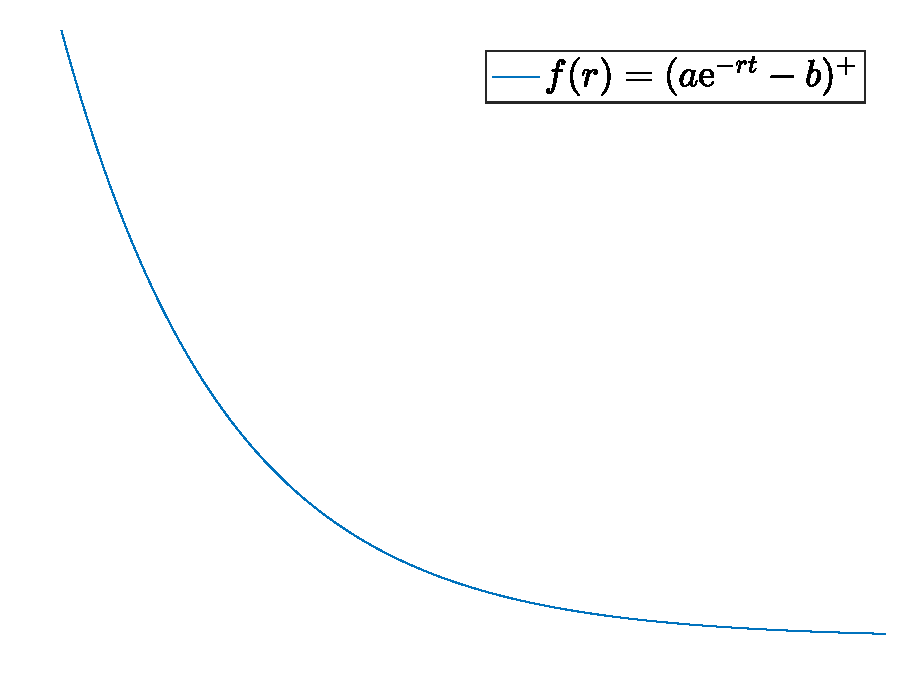
\includegraphics[scale=0.4]{7.17.eps}
    \end{figure}
    \item \sol\\
    没有绝对的凹凸性.
\end{enumerate}
\clearpage